\documentclass{article}
\usepackage[utf8]{inputenc}
\title{Lecture 5 kernel methosd}
\author{wbg231 }
\date{December 2022}
\newcommand{\R}{$\mathbb{R}$}
\newcommand{\B}{$\beta$}
\newcommand{\A}{$\alpha$}
\newcommand{\D}{\Delta}

\newcommand{\avector}[2]{(#1_2,\ldots,#1_{#2})}
\newcommand{\makedef}[2]{$\textbf{#1}$:#2 }
\usepackage{tikz,graphicx,hyperref,amsmath,amsfonts,amscd,amssymb,bm,cite,epsfig,epsf,url}

\begin{document}

\maketitle

\section*{introduction}
\begin{itemize}
\item \href{https://nyu-ds1003.github.io/mlcourse/2023/lectures/lec05/05.pdf}{slides link}
\section{feature maps}
\subsection{the input space X}
\item our general learning theory setup makes no assumptions about the input space $\mathcal{X}$
\item but all the linear methods we have build so far assume that $\mathcal{X}=\mathbb{R}^{d}$  (including ridge, lasso, and SVM)
\item out hypothesis space for these questions was all affine functions in $\mathbb{R}^{d}$ $$\mathcal{F}=\{w\rightarrow W^tx+b|w\in \mathbb{R}^{d}, b\in \mathbb{R} \}$$
\item what if we want to use inputs that are not within real numbers, like we are dealing with text documents, images, recordings, DNA
\item but everything in a computer needs to be represented by a sequence of Numbers,
\item the ith entry of each sequence should have the same meaning, for example in real numbers $x_[i]$ represents the coordinate in the i direction
\item all sequences should have the same meaning.
\subsection{feature extraction}
\item call a feature extractor a mapping of an input from $\mathcal{X}$ to a vector in $\mathbb{R}^{d}$  
\subsection{linear models with explicit feature maps }
\item in this set up we assume the feature space is $\mathcal{X}$
\item and we introduce feature map $\phi:\mathcal{X}\rightarrow \mathbb{R}^{d}$
\item the feature map maps features into the feature space $\mathbb{R}^{d}$
\item the hypothesis space is the affine functions on the feature space ie $$\mathcal{F}=\{ x\rightarrow w^{t}\phi(x)+b|w\in \mathbb{R}^{d}, b\in \mathbb{R}  \}$$
\item so in other words our hypothesis space is all affine functions that on the feature map. so that just means it must be a shifted plus scaled combination of what ever we put into the feature map 
\subsection{two class problem}
\item 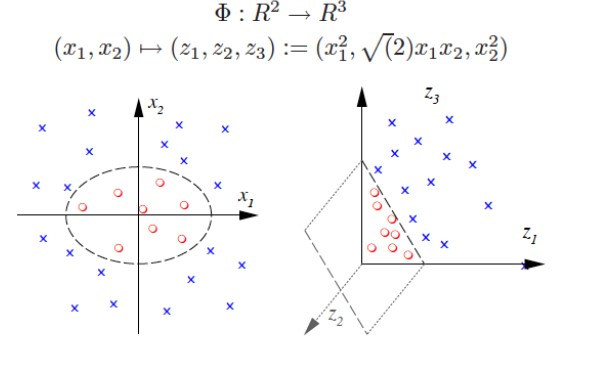
\includegraphics[width=10cm]{lecture_notes/lecture_5/immage/l_5_1.jpg}
\item suppose our data in $\mathbb{R}^{d}$ looks like the graph on the right. 
\item but if set a feature map to be $\phi(x)=(x,y,x^2+y^2)$ then there exists some mapping $w_1x+w_2y+w_3(x^2+y^2)$that we get linearly separable data in the new space (the graph on the left) then if we project that back into our original space it looks like our  boundary is a circle :)
\item \href{https://www.youtube.com/watch?v=3liCbRZPrZA}{here is a video on it}
\subsection{Expressivity  of the hypothesis space}
\item for linear models to grow the the hypothesis space we need to add more features
\item we say that a larger hypothesis space is More expressive
\section{handling nonliterary with linear methods}
\subsection{example task}
\item suppose we are predicting health care outcomes 
\item our general approach is to extract every feature that may be important 
\item these could include height weight blood pressure etc
\subsection{feature issues for linear predictors}
\item for linear predictors it is important how feature's are added; the relationship between a feature and a label may not be linear. there may be a complex dependency among features 
\item three types of non-linearity's can cause problems. non-monotonic, saturation, interactions between features 
\subsection{non-monotonicity}
\item suppose we have a feature map $\phi(x)=[1, temperture(x)]$ this notation means our affine function can be $w_1(1)+w_2($temperature(x)
\item our action is predict health score $y\in \mathbb{R}$
\item our hypothesis space is all afine functions of temperature 
\item the issue is that health is not an affine function of temperature, 
\item affine functions (are monotonic) that is adding more of x should always increase or decrease y
\item but in temperature both extremes are bad. 
\item there are two ways to deal with this 
\begin{itemize}
    \item we could define a super specific input space that fits the domain, but this  requires a lot of domain knowledge. so we could design something like $\phi(x)=[1, (temp(x)-37)^2]$
    \item we could think less but put in more that is we could define a feature map $\phi(x)=[1,temp(x),temp(x)^2]$ features should be simple building blocks that can be pieced tougher
\end{itemize}
\subsection{saturation: the issue}
\item suppose our goal is to find product rel event to a users query 
\item our input is a product X
\item our action is to score the relevance of x to the users query 
\item a feature map such as $\phi(x)=\{1,N(x)\}$ where n is the number of people who buy product x 
\item we expect a monotonic relationship between n(x) and relevance but also diminishing returns. (that is if you buy 2 units of bread and one unit of water, bread is more important but not twice as important)
\subsection{saturation: solution}
\item we can smooth these changes with non-linear feature transforms such as $\phi(x)=[1,log(1+n(x))]$ log is good at dealing with large ranges. 
\item one could also create a discrete feature space such as $\phi(X)=[1, 1(0\leq N(x)\leq 10), 1(10\leq n(x)\leq 100)...]$
\item so that is we way the number of items differently depending on there bin 
\subsection{interactions: the issue}
\item suppose our input is patient information x
\itme our action to assign a real values health score y
\item if we have the feature map $\phi(x)=[height(x),wieght(x)]$ this may fail to capture the relationship as weight relative to height is an important indicator of health outcomes, that is there is an interaction 
\subsection{interactions solution}
\item approach 1: have domain info and specifically design a feature map for the interaction interaction 

\item approach 2 just include all second order features that is $phi(x)=[1.h(x),w(x),h^2(x), w^2(x), h(X)w(x)]$ where $h(X)w(x)$ is our cross term. this is nice as it does not require domain knowledge.  
\item  issue
\begin{itemize}
    \item suppose we start with $x=(1,x_1,...x_d)\in \mathbb{R}^d$
    \item consider all monomials of degree $M: x_1^p_1..x_d^p_d$ with $p_1+..+p_d=m$  so for instance if M=2 and x is in r 2 we would have $xy,x^2,y^2$
    \item so we would end up with \begin{pmatrix}m+d+1\\m
    \end{pmatrix} features if we include all monomials 
    \item this means using this approach will grow our data matrix very quickly
\end{itemize}
\subsection{ big feature spaces}
\item very large feature spaces both tend to over fit and are computationally expensive
\item we can deal with the overfititng with regularization and try to deal with computational and memory issues with kernel methods
\section{the kernel trick}
\subsection{SVM with explicit feature map}
\item recall that the standard SVM problem for the input space $X\in \mathbb{R}^D$ is  $min_{w\in \mathbb{R}^d}\frac{1}{2}||W||^2+\frac{c}{n}\Sigma_{i=1}^{n}max(0,1-y_iw^tx_i)$
\item we can expand this to given an arbitrary feature space X as long as we have a  feature map $\phi:X\rightarrow R^{D}$ which makes the svm $$min_{w\in \mathbb{R}^d}\frac{1}{2}||W||^2+\frac{c}{n}\Sigma_{i=1}^{n}max(0,1-y_iw^t\phi(x_i))$$
\item this can be computationally expensive if d is large
\item however recall that the SVM dual problem can expressed as $$max \Sigma_{i=1}^{n}\alpha_{i}-\frac{1}{2}\Sigma_{i,j=1}^{n}\alpha_i\alpha_{j}y_iy_j\phi(x_i)^{t}\phi(x_i) \quad st \quad  \Sigma_{i=1}^{n}\alpha_{i}y_{i}=0, \alpha_{i}\in [0,\frac{c}{n}]$$
\item if $\alpha^{*}$ is the optimal value then $w^{*}=\Sigma_{i=1}^{n}\alpha_{i}y_i\phi(x_i)$ and $\hat{f}(x)=\Sigma_{i=1}^{n}\alpha_{i}^{*}y_i\phi(x_i)^t\phi(x)$
\item notice here that both in our training and inference we only see $\phi(x)$ in an inner product with  another $\phi(x_i)$
\subsection{compute inner product}
\item suppose we are on 2d data, and we have a degree 2 monomial $\ph(x):\mathbb{R}^{2}\rightarrow \mathbb{R}^{3}$ such that $(x,y)\rightarrow (x_1^2, \sqrt{2}xy,y^2)$
\item notice in this case for any x,y we can write $\phi(x)^t\phi(y)=(x_1y_1)^2+2(x_1y_1)(x_2y_2)+(x_2y_w)^2=(x_1y_1+w_2y_2)^2=(x{t}x)^{2}$
\item in other words we can Calcutta the inner product $<\phi(x)\phi{y}>=\phi(x)^{t}\phi{y}$ with only the original input x we don't actually need $\phi$
\item monomials of degree 2 $
\phi:(x_1,x_2)\Rightarrow (1,\sqrt{2}x_1, \sqrt{2}x_2, x_1^2 , x_2^2, \sqrt{2}x_1x__2)$
\item so lets compute the inner product of this thing backwards $$(1+x^{t}y)^2=(1+(x_1y_1+x_2y_2))+(1+(x_1y_1+x_2y_2))=1+2x_1y_1+2x_2y_2+x_1^2y_1^2+2x_1y_1x_2y_2+x_2^2y_2^2\\=\phi(x)^t\phi(y)$$
\item so in other words this feature map can also be understood just in terms of its input space 
\item more generally feature maps producing monomial up to degree-p we have $$\phi(x)^{t}\phi(y)=(1+x^ty)^{p}$$
\item  so the \textbf{the kernel TRICK} is that we do not need $\phi(x)$ to calculate the inner product just x
\item this is help full because if we are using explicit features for the monomial case that would be $O(D^{n})$ ie exponential time but in the original feature space x that we can use for explicit computation of time complexity is $O(d)$
\section{kernel functions}
\subsection{the kernel function}
\item given input space $\mathcal{X}$
\item feature space $\mathcal{H}$ a Hilbert space ( a Hilbert space is a vector space $V$ with an inner product $<>$ such that the norm defined as  $|v|=\sqrt{<v,v>}$ turns V into a complete metric space. Recall a metric space is just a set (in this case V) with a distance metric in this case $(|V|)$. and a complete metric space more or less means that every Cauchy sequence ie a sequence a such that $lim_{m,n}_{\rightarrow\infty}d(a_n,a_m)=||a_n,a_m||=0$ converges that is the limit of the sequence is defined. in other words as any two vectors a,b in our vector space v get infinitely close to each other in the limit it must be the case that  they equal one another. All this more or less means that we just have a well "behaved"  vector space with a norm induced by some inner product.  \href{https://mathworld.wolfram.com/HilbertSpace.html}{metric space}) as a separate point this whole analysis is kind of unnecessary in the context of computer science, since regardless of the feature space for instance images we need to be able to represent them with real Numbers, and real numbers with euclidean distance are a Hilbert space (so in other words we will never not be in a Hilbert space in comp sci)
\item then we have a feature map $\phi:\mathcal{X}\\rightarrow \mathcal{H}$
\item the kernel function corresponding to $\phi$ is $$k(x,y)=<\phi(x), \phi(y)>$$ where $<*,*>$ is the inner product associated to $\mathcal{H}$
\item often we can evaluate $K<x,y> $ with out explicitly computing $\phi(x),\phi(y)$
\item when can we use the kernel trick
\subsection{some method can be Kernelized}
\item a method can be Kernelized if  every feature vector $\phi(x)$ only appears inside an inner product with another feature vector $\phi(y)$. this must be the case both in the optimization and prediction functions 
\item  so for instance in svm our optimization problem is 
 $$max \Sigma_{i=1}^{n}\alpha_{i}-\frac{1}{2}\Sigma_{i,j=1}^{n}\alpha_i\alpha_{j}y_iy_j\phi(x_i)^{t}\phi(x_i) \quad st \quad  \Sigma_{i=1}^{n}\alpha_{i}y_{i}=0, \alpha_{i}\in [0,\frac{c}{n}]$$
\item and our prediction problem is $\hat{f}(x)=\Sigma_{i=1}^{n}\alpha_{i}^{*}y_i\phi(x_i)^t\phi(x)$
\item thus the svm can be kernelized
\subsection{the kernel matrix}
\item the kernel matrix for a kernel k on input data $x_1...x_n\in \mathcal{X}$ is $$K=(k(x_i,s_j))_{i,j}=\begin{pmatrix}
    k(x_1,x_1)&...&k(x_1,x_n)\\
    ...&...&...\\
    k(x_n,x_1)&...&k(x_n,x_n)
\end{pmatrix} \in \mathbb{R}^{n\times n}$$ 
\item this is often called the gram matrix in ml 
\item the kernel matrix summarizes all information we need about the training input $x_1...x_n$ to solve a kernelized  optimization problem 
\item so thus in the kenelized SVM problem we can be written as $$=max \Sigma_{i=1}^{n}\alpha_{i}-\frac{1}{2}\Sigma_{i,j=1}^{n}\alpha_i\alpha_{j}y_iy_jK_{i,j} \quad st \quad  \Sigma_{i=1}^{n}\alpha_{i}y_{i}=0, \alpha_{i}\in [0,\frac{c}{n}]$$ 
\subsection{kernel methods}
\item given a kernealized ml algorithm (that is all $\phi(x)$ only show up as $\phi(x)^{t}\phi(y)$
\begin{itemize}
    \item we cab swap the inner product with our kernel function $k(x,y)$
    \item the new kernel may correspond to a very high dimensional feature space
    \item once the kernel matrix is computed the computation cost depends on the number of data points n rather than the dimension of the new feature space d
    \item this is useful when $d>>n$ (that is the dimension of our feature space is much larger than the number of data points)
    \item it is important however to note that computing the kernel matrix may still dependence on d so part of the trick is getting around the $O(d)$ dependence 
\end{itemize}
\section{example kernels}
\subsection{similarity scores}
\item think of kernels $k(x,y)$ as similarity scores (this makes sense as H is a metric space and K is a function of our distance metric and the distance between two vectors can be thought of as there similarity, like how the dot product of vectors in $\mathbb{R}^{d}$ more or less tell us how much the vectors are pointing in the same direction 
\item so for different contexts we can design kernels to be similarity scores without thinking about explicit feature maps (like string distance) 
\item how do we know our kernel correspond to an inner product in some feature space? 
\subsection{how to get kernels}
\item we can explicit design feature maps and define a kernel as $k(x,y)=\phi(x)^t\phi(y)$
\item or we can define a kernel function as as a similarity score k(x,y) and verify it corresponds to $<\phi(x),\phi(y)>$ for some feature map $\phi$
\subsection{linear algebra positive semi definite matrix}
\item a matrix M is psd if $\forall x\in \mathbb{R}^{n}$ $$x^tMX\geq 0$$
\item the following are necessary and sufficient for a symmetric matrix m to be positive semi definite
\begin{itemize}
    \item M can be factorized as $M=R^TR$ for some matrix R
    \imte all eigenvalues of m are greater than or equal to zero
\end{itemize}
\subsection{positive definite kernel}
\item a symmetric function $k: \mathcal{X}:\mathcal{X}\rightarrow R$ is positive finite on $\mathcal{X}$ if for any finite set $\{x_1..x_n\}\subset\mathcal{X}$ the kennel matrix on this set $$K=(k(x_i,s_j))_{i,j}=\begin{pmatrix}
    k(x_1,x_1)&...&k(x_1,x_n)\\
    ...&...&...\\
    k(x_n,x_1)&...&k(x_n,x_n)
\end{pmatrix} \in \mathbb{R}^{n\times n}$$  is positive semi definite 
\item symmetric matrix $K(x,y)=K(y,x)$
\item the kernel matrix needs to be positive semi definite for any finite set of points 
\item this is equivalent to saying $\Sigma_{i=1}^{n}\Sigma_{j=1}^{n}\alpha_{i}\alpha_{i}K(x_i,x_j)\geq 0$ given $\alpha \in \mathbb{R}$
\subsection{mercer's tearoom }
\item mercers theorem states that a symmetric function $k(x,y)$ can be expressed as an inner product $$K(x,y)=<\phi(x),\phi(y)>$$ for some $\phi\iff K(x,y)$ us positive definite 
\item probing a function is positive definite is typically not easy 
\item but we can construct new kernels form valid kernels 
\subsection{generating new kernels form old}
\item suppose $k,k_1,k_2:\mathcal{X}\times \mathcal{X}\rightarrow \mathbb{R}$ are postive definte kernels then so are the following. 
\begin{enumerate}
    \item $k_{new}(s,y)=\alpha k(x,y) $ if $\alpha\geq 0$
    \item $k_{new}(x,y)=k_1(x,y)+k_2(x,y)$
    \item $k_{new}(x,y)=k_1(x,y)k_2(x,y)$
    \item $k_{new}(x,y)=k(\phi(x), \phi(y))$ for any function $\phi$
    \item $k_{new}(x,y)=f(x)f(y)$ for any function $f(*)$
\end{enumerate}
\subsection{linear kernel}
\item input space $X=\mathbb{R}^{d}$
\item feature space $\mathcal{H}=\mathbb{R}^{d}$ with a standard inner product 
\item feature map $\phi(x)=x$
\item kernel $k(x,y)=x^{t}y$ 
\subsection{quadratic kernel}
$X=\mathbb{R}^{d}$
\item feature space $\mathcal{H}=\mathbb{R}^{D}$ where $D=d+\begin{pmatrix}
    d\\2
\end{pmatrix}$ 
\item the feature map $\phi(x)=[x_1...x_d, x_1^2...x_d^2...\sqrt{2}x_1x_2...\sqrt{2}x_{d-1}x_{d}]^{t}$
\item then for $\forall x,y\in \mathbb{R}^{d} $ we have $$k(x,y)=<\phi(x),\phi(y)>=<x,y>+<x,y>^{2}$$
\subsection{polynomial kernel kernel}
$X=\mathbb{R}^{d}$
\item the kernel function $K(x,y)=(1+<x,y>)^M$
\item this corresponds to the feature map $\phi$ with all minimal up to degree m 
\item for any M computing the kernel has the sme computation cost 
\itme the cost of the inner product computation however grows exponentially in n 
\subsection{RBF}
\item let our input space be $\mathcal{X}=\mathbb{R}^{d}$ such that $$K(x,y)=e(-\frac{||x-y||^{2}}{2\sigma^{2}})$$
\item where $\sigma^2$ is known as a band with parameter 
\item the rbf kernel is the most popular linear kernel 
\item it kind of co responds to a polynomial kernel of degree infinite if you explicit write out the sum 
\subsection{remaining questions}
\item our current recepie is 
\begin{itemize}
    \item recognize kernalized problem where $\phi$ only occurs within inner product $\phi^{t}(x)\phi(y)$
    \item pick a kernel function (like a similarity score)
    \item compute the kernel matrix (nxn) where n is the data set size
    \item optimize the model t make predictions by accessing the kernel matrix 
\end{itemize}
\item the next question is when can we apply generalization 
\section{representer theorem}
\subsection{SVM observation}
\item  recall from earlier our  svm our optimization problem is 
 $$max \Sigma_{i=1}^{n}\alpha_{i}-\frac{1}{2}\Sigma_{i,j=1}^{n}\alpha_i\alpha_{j}y_iy_j\phi(x_i)^{t}\phi(x_i) \quad st \quad  \Sigma_{i=1}^{n}\alpha_{i}y_{i}=0, \alpha_{i}\in [0,\frac{c}{n}]$$
\item and our prediction problem is $\hat{f}(x)=\Sigma_{i=1}^{n}\alpha_{i}^{*}y_i\phi(x_i)^t\phi(x)$
\item thus the svm can be kernelized, meaning that $w^{*}$ is a linear combination of our training input and thus $w^{*}\in span(x_1...x_n)$
\subsection{ridge observation}
\item recall that ridge regression sollution is $$w^{*}=armin_{w\in \matbb{R}^D}\frac{1}{n}\Sigma_{i=1}^{n}(w^{t}x_i-y_i)^2+\lambda||w||_{2}^2$$
\item which has closed form solution $W^{*}=(X^{T}X+\lambda I)^{-1}X^Ty$ where X is the design matrix with $x_1..x_n$ as rows
\item notice that we can write $W^{*}=(X^{T}X+\lambda I)^{-1}X^Ty=X^{t}(\frac{1}{\lambda}y-\frac{1}{\lambda}Xw^{*})=X^{t}\alpha^{8}=\Sigma_{i=1}^{n}\alpha_{i}x_i\in span(x_1...x_n)$
\item that is in both the case of ridge and svm our solution $w^{*}$ is a linear combination of our training data and thus in the span of our training data 
\subsection{parameterize ridge}
\item as we know $W^{*}\in span(x_1...x_n)\subset R^{d}$ we can rewrite our ridge solution as$$w^{*}=armin_{w\in \matbb{R}^D}\frac{1}{n}\Sigma_{i=1}^{n}(w^{t}x_i-y_i)^2+\lambda||w||_{2}^2=armin_{ w\in span(x_1...x_n)}\frac{1}{n}\Sigma_{i=1}^{n}(w^{t}x_i-y_i)^2+\lambda||w||_{2}^2$$ 
\item further $w\in span(x_1..x_n)\Rightarrow W^{*}=\Sigma_{i=1}^{n}x_i\alpha_i=X^{t}\alpha$ for some $\alpha \in \mathbb{R}^{n}$
\item so thus our original problem can $w^{*}=armin_{w\in \matbb{R}^D}\frac{1}{n}\Sigma_{i=1}^{n}(w^{t}x_i-y_i)^2+\lambda ||W||_{2}^{2}$ can be written as $$\alpha^{*}=armin_{\alpha \in \matbb{R}^{n}}\frac{1}{n}\Sigma_{i=1}^{n}(X^{t}\alpha )^{T}x_i-y_i)^2+\lambda ||X^{t}\alpha||_{2}^{2}$$
\item then we can naturally get $w^{*}$ as $w^{*}=X^t\alpha^*$
\item so notice that the dimension of our problem when working with $W^{*}\in \mathbb{R}^{d}$ is d (ie the number of features), but working with $\alpha^{*}\in \mathbb{R}^{n}$ it is n (ie the number of data points).
\subsection{consider very large feature spaces}
\item suppose our feature space so 300 million dimension (like for instance if we are modeling high order monomial interactions)
\item suppose we also have a set of 300,000 training examples
\item in the original formulation we solve a 300 million dimensional optimization problem 
\item in the reparameterized   $\alpha$ problem we solve a 300,000 dimensional optimization problem 
\item  so reparameterization  is good when we have many more features than data 
\section{inner products and Hilbert spaces}
\subsection{Hypothesis  space so far }
\item we have an arbitrary input space $\mathcal{X}$
\item we make no assumptions on our hypothesis space $\mathbf{F}$
\item we have a feature map $\phi:\mathcal{H}\rightarrow \mathcal{F}$ which does not have to be linear 
\item our feature space is $\mathcal{H}=\{f:\mathbf{X}\rightarrow \mathbb{R}|f(x)=w^{t}\phi(x)\} $
\subsection{inner product space}
\item an inner product space (or pre Hilbert space) is a vector space $V$ with an inner product which is mapping $$<*,*>:V\times V\rightarrow \mathbb{R}$$
\item where the inner product is symmetric linear and positive definite. (that is an inner product)
\subsection{show dot product is inner product}
\item first lets check symmetry $<x,y>=X^{t}y=(X^{t}y)^{T}=y^{t}x=<y,x>$
\item next lets check linearity $<ax+b,z>=(ax+b)^{t}z=x^{t}a{t}z+b^{t}z=a(x^{t}z)+b^{t}z=a<x,z>+<b,z>$
\item next we want to show postive defininteness so first we need to show $<x,x>\geq 0$ this makes sense as $<x,x>=x^{t}x=\Sigma_{i=1}^{n}x_{i}^2\geq 0$
\item to finish positive definiteness we want to show that $<x,x>=0\iff x=0$ so assume that x=0 then $<x,x>=\Sigma_{i=1}^{n}x_i^2=(n)0^{2}=0$ thus $<x,x>=0\leftarrow x=0$ 
\item next assume that $<x,x>=0$ this means that $\Sigma_{i=1}^{n}x_i^{2}=0$ $x_i^2\geq 0$ always so only holds if all $x_i=0\rightarrow X=0$
\item thus we have $<x,x>\geq 0$ and $<x,x>=0\iff x=0$ meaning that it is positive definite 
\item thus the dot product is an inner product 
\subsection{norm from an inner product}
\item the inner product is nice because it allows us to get a grasp of size distance and angle for a vector space. from this we can define a norm on that vector space as $$|x|=\sqrt{<x,x>}$$
\subsection{orthogonality}
\item for any vectors $x,y\in\mathbb{R}^{d} $ $x\perp y\iff <x,x>=0$ that is they are orthogonal 
\item a vector $x$ is orthogonal to a set S if $\forall s\in S <X,s>=0$ written as $x\perp S$
\subsection{Pythagoras theorem}
\item suppose $x\perp y$ then $||x+y||^2=<x+y,x+y>=(x+y)^{t}(x+1)=x^tx+x^ty+y^tx+y^ty={x^tx+y^ty}=|x|+|y|=||x||+|y|$
\item so the theorem is$x\perp y\rightarrow ||x+y||^{2}\leq ||x||^{2}+||y||^2$
\subsection{Hilbert space }
\item a pre Hilbert space is a vector space with an inner product 
\item a Hilbert space is a complete metric space meaning all Cauchy sequences converge to a point in the space
\item so a Hilbert space is a complete inner product space, that is a complete metric space on some vector space and inner product function
\section{representer theorem}
\subsection{general SVM}
\item the SVM objective function is written as $min_{w\in \mathbb{R}^{d}}\frac{1}{2}||w||^2+\frac{c}{n}\Sigma_{i=1}^{n}max(0,1-yi[<w,x_i>]$
\item the generalized objective function for the SVM is $min_{w\in \mathcal{H}}R(||w||)+L(<w,x_1>...<w,x_n>)$ 
\item where $x_1..x_n\in \mathcal{H}$ for some Hilbert space $\mathcal{H}$  that is our tiring data is in the Hilbert space
\item ||*|| is the norm corresponding to the inner product of $\mathcal{H} $ that is $||*||=\sqrt{<*,*>}$
\item we have regularization term R where R is a function such that $R:[0,\infty]\rightarrow \infty$ that is it takes only positive wight norms and regularizes them pushing for the magnitude of the weight vector
\item and we have loss term  $L:\mathbb{R}^{n}\rightarrow \mathbb{R}$
\section{general objective function for linear hypothesis space }
\item suppose we restrict our self to a linear hypothesis space $\mathcal{F}$
\item then in general we can write our objective as $min_{x\in \mathcal{H}}R(||w||)+L(<w,x_1>...<w,x_n>)$
\item notice this function does not change if we map $x_i$ to a feature space
\item our predictions (or score are given by $f:W\rightarrow \mathcal{F}:f(w)=w^{t}x=<w,x?$ notice that f is linear in w 
\item if we set $R=\frac{1}{2}$ and $L(w)=\frac{c}{n}max(0,1-yw^tx_i)$ then we have the svm 
\item if we set $R(||w||)=\lambda(||w||)^{2}$ and $L(w)=(y-Xw)^{t}(w-Xw)$ then we have ridge 
\item this form will not however hold for lasso regression as $\ell_{1}$ norm does not correspond to an inner product 
\subsection{representer theorem}
\item general we can write our objective as $min_{x\in \mathcal{H}}R(||w||)+L(<w,x_1>...<w,x_n>)$
\item the respresenter theorem tells us we can look for $w^{*}$ in the span of our data ie $$w^{*}=min_{w\in span(x_1..x_n)}R(||W||)+L(<w,x_1>...<x,x_n>)$$
\item so as $w\in span(x_1...x_n)$ we can write $w^{*}=\Sigma_{i=1}^{n}\alpha_ix_i$ for some $\alpha$
\item thus we can reparameterize  our objective as $$\alpha^{*}=argmin_{\alpha\in\mathbb{R}^d}R(||\Sigma_{i=1}^{n}\alpha_ix_i||)+L(<\Sigma_{i=1}^{n}\alpha_ix_i,x_1>...<\Sigma_{i=1}^{n}\alpha_ix_i,x_n>)$$
\item so notice here that our prediction and objective functions are in terms of $<x,x^{i}>$ thus we can apply our kernel trick to anything that meets this generalized objective form 
\subsection{representer theorem formal}
\item the representer theorem say 
\begin{itemize}
    \item let $J(w)=R(|w|)+L(<w,x_1)...<w,x_n>)$
    \item where $w,x_1...x_m\in \mathcal{H}$ for some some Hilbert space $\mathcal{H}$ 
    \item $||x ||$  is the norm corresponding to the inner product on that Hilbert space$ \mathcal{H}$ that is $||w||=\sqrt{<w,w>}$
    \item we have regularization term R where R is a function such that $R:[0,\infty]\rightarrow \infty$ is non decreasing 
\item and we have loss term  $L:\mathbb{R}^{n}\rightarrow \mathbb{R}$ is arbitrary
\item then j has a minimizer in the span of the input data that is $w^{*}=\alpha x=\Sigma_{i=1}^{n}\alpha_{i}x_{i}\in span(x_1...x_n)$
\end{itemize}
\section{Reparameterizing our generalized objective function}
\subsection{re write the objective function}
\item defined the training score of function s as $s:\mathcal{R}^{d}\rightarrow \mathcal{R}$ by $s(w)=\begin{pmatrix}
    <w,x_1>\\..\\<w,x_n>
\end{pmatrix}$ that is our score function is a column vector with the inner product of our found weights and all training points 
\item then we can write $J(w)=R(|w|)+L(<w,x_1)...<w,x_n>)=R(|W|)+L(s(w))$ where $L:R^{n\times1}\rightarrow\mathbb{R}$
\item assuming j meets the requirements we can use the repent theorem to say that to find the min of j(W) we only need to look over $w=\Sigma_{i=1}^{n}\alpha_{i}x_{i}\in span(x_1..x_n)$
\item allowing us to write $J_{0}(\alpha)=R(|\Sigma_{i=1}^{n}\alpha_{i}x_{i}|)+L(s(\Sigma_{i=1}^{n}\alpha_{i}x_{i}))$ over $\alpha = (\alpha_1...\alpha_n)^{t}\in \matbb{R}^{n\times 1}$
\subsection{simpify the norm}
\item note taht we can write our norm as $||w||=||\Sigma_{i=1}^{n}\alpha_{i}x_{i}||$
\item and furhter $||w||^{2}=||\Sigma_{i=1}^{n}\alpha_{i}x_{i}||^{2}=<\Sigma_{i=1}^{n}\alpha_{i}x_{i},\Sigma_{i=1}^{n}\alpha_{i}x_{i}>=\Sigma_{i,j=1}^{n}\alpha_{i}\alpha_{j}<x_i,x_j>$
\item note that this expression involves $n^2$ inner products between all Paris of input vectors $x_i$
\item we can rite this using a kernel matrix 
\subsection{gram matrix for a dot product}
\item consider $x\in R^{d\times 1}$ with the dot product
\item let $X\in \mathbb^{R\times d}$ by the dissing matrix with each input vector as a row $X=\begin{pmatrix}
    x_1^t\\..\\x_n^t
\end{pmatrix}$
\item tehn we can write our ghram or kernel matrix as $$K=\begin{pmatrix}
    x_1^{t}x_1&...&x_1^{t}x_n\\
    ... &...&...\\
    x_n^{t}x_1&...&x_{n}^{t}x_{n}^{t}
\end{pmatrix}=\begin{pmatrix}
    x_1^t\\..\\x_n^t
\end{pmatrix}\begin{pmatrix}
    x_1&..&x_n
\end{pmatrix}=XX^{T}$$
\subsection{simplifying the norm }
\item given $w=\Sigma_{i=1}^{n}\alpha_{i}x_{i}$
\item $||w||^{2}=||\Sigma_{i=1}^{n}\alpha_{i}x_{i}||^{2}=<\Sigma_{i=1}^{n}\alpha_{i}x_{i},\Sigma_{i=1}^{n}\alpha_{i}x_{i}>=\Sigma_{i,j=1}^{n}\alpha_{i}\alpha_{j}<x_i,x_j>=\alpha^{t}K\alpha$
\subsection{simplifying the training score }
\item given $w=\Sigma_{i=1}^{n}\alpha_{i}x_{i}$
\item the score is $<x,x_{j}>=\alpha_{i}x_{i}=<\Sigma_{i=1}^{n}\alpha_{i}x_{i},x_j>=\Sigma_{i=1}^{n}\alpha_{i}<x_{i}, x_j>$
\item thus we can writing the training  score vector $s(w)=s(\Sigma_{i=1}^{n}\alpha_{i}x_{i})=\begin{pmatrix}
    \Sigma_{i=1}^{n}\alpha_{i}x_{1}\\..\\\Sigma_{i=1}^{n}\alpha_{i}x_{n}
\end{pmatrix}=\begin{pmatrix}
    \alpha_1<x_1,x_1>+...+\alpha_n<x_n,x_1>\\...\\\alpha_1<x_n,x_1>+...+\alpha_n<x_n,x_n>
\end{pmatrix}=\\\begin{pmatrix}
    <x_1,x_1>+...+<x_n,x_1>\\...\\\<x_n,x_1>+...+<x_n,x_n>
\end{pmatrix}\begin{pmatrix}
    \alpha_1\\...\\\alpha_n
\end{pmatrix}=K\alpha$
\subsection{parameterized objective }
\item putting everything tooter allows us to write $j_{0}(\alpha)=R(||\Sigma_{i=1}^{n}\alpha_ix_i||)+L(s(\Sigma_{i=1}^{n}\alpha_ix_i))=R(\sqrt{\alpha^{t}K\alpha})+L(k\alpha)$ which can be minimized over all $\alpha\in\mathbb{R}^{n}$
\item so keep in mind that all information about the training set $x_1...x_n$ is held in our gram matrix K
\item we are also now optimizing over n dimensions instead of k. so this is good if $d>>n$
\subsection{dramatizing predictions}
\item if we have $\alpha^{*}=argmin_{\alpha \in \mathbb{R}^{n}}R(\sqrt{\alpha^{t}K\alpha})+L(k\alpha)$
\item then we know $w^{*}=\Sigma_{i=1}^{n}\alpha_ix_i$ is our solution to $argmin_{w\in \mathcal{H}}R(||W||)+L(<w,x_1>...<w,x_n>)=J(w)$
\item and thus our prediction for a new point $x\in \mathcal{H}$ is $$\hat{f}(x)=w^{*t}x=<w^{*},x>=\Sigma_{i=1}^n\alpha_{i}^{*}<x_i,x>$$
\item thus to make new predictions we may need to touch all training inputs which could be costly 
\item  we can define the column vector for any $x\in \mathcal{H}$ as $$K_{x}=\begin{pmatrix}
    <x_1,x>\\...\\<x_n,x>
\end{pmatrix}$$
\item  allowing us to write the prediction of a new point $x\in\mathcal{H}$ as $$\hat{f}(x)=w^{*t}x=<w^{*},x>=\Sigma_{i=1}^n\alpha_{i}^{*}<x_i,x>=K_{x}^{t}\alpha^{*}$$
\end{itemize}
\subsection{Kernelization}
\item  a method is kernelized if for every feature vector $\phi(x)$ only appears in an inner product with another feature vector $\phi(x')$. this applies both to the optimization and prediction problems. 
\item in this set up finding  $\alpha^{*}\in armin_{\alpha\in \mathbb{R}^{n}}R(\sqrt{\alpha^{t}K\alpha }) +L(K\alpha)$ and making predictions $\hat{f}(x)=K_{x}^{t}\alpha^{*}$ is a kernelization of finding $w^{*}\in argmin_{w\in\mathcal{H}}R(||w||)+L(<w,\phi(x_1)>...<w,\phi(x_n)>$ and making predictions with $\hat{f}(x)=<w^{*},\phi(x)>$

\end{document}
